% -*- mode: latex; mode: flyspell -*-

%%% Local Variables:
%%% TeX-master: "mu2e-36575"
%%% End:

%%%%%%%%%%%%%%%%%%%%%%%%%%%%%%%%%%%%%%%%%%%%%%%%%%%%%%%%%%%%%%%%%%%%%%%%%%%%%%
\section{Particle identification}
% {\blue lowercase title words after first word}

For muons, the momentum region around 100 MeV/c for muons the region where the transition 
the non-relativistic to the ultra-relativistic regime is happening.
As shown in Figure \ref{fig:pid_ep_dt}, distributions of important particle ID variables 
for 92 MeV/c and 105 MeV/c muons are quite different. Therefore it makes sense to optimize
the particle ID algorithms for the \MuToEm\ and \MuToEp\ conversion searches separately.

\begin{figure}[H]
\hspace{-0.6in}
  \begin{tikzpicture}
    \node[anchor=south west,inner sep=0] at (0,0.) {
      % \node[shift={(0 cm,0.cm)},inner sep=0,rotate={90}] at (0,0) {}
      % \makebox[\textwidth][c] {
      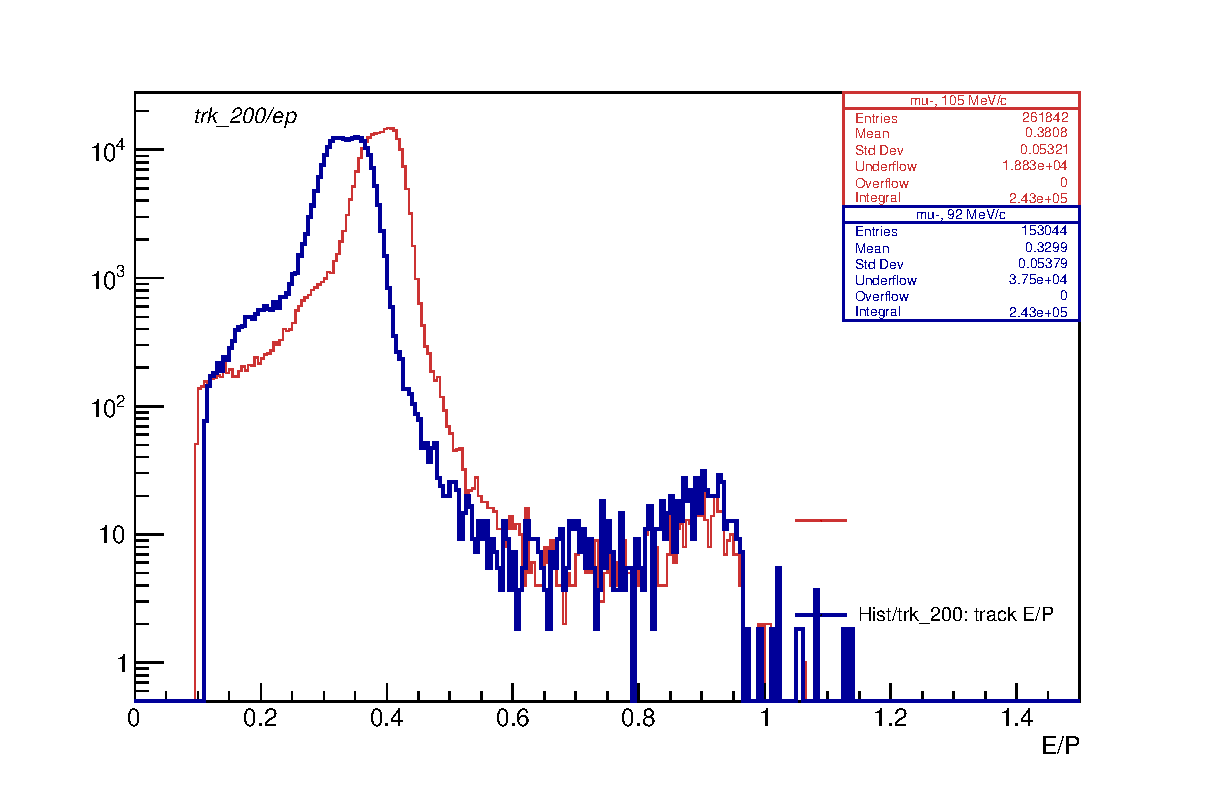
\includegraphics[width=0.64\textwidth]{figures/pdf/figure_00321_su2020_track_ana_trk_200_ep}
      % }
    };
    \node[anchor=south west,inner sep=0] at (10.5,0.) {
      % \node[shift={(0 cm,0.cm)},inner sep=0,rotate={90}] at (0,0) {}
      % \makebox[\textwidth][c] {
      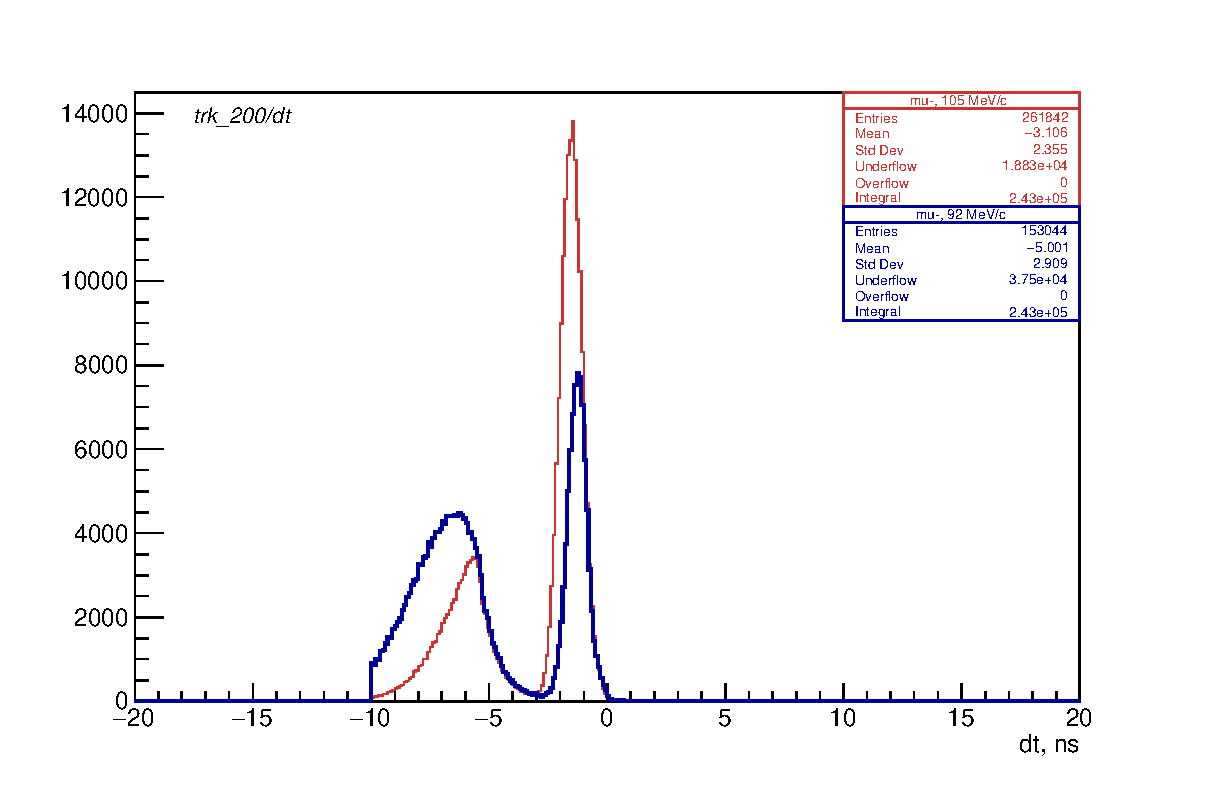
\includegraphics[width=0.64\textwidth]{figures/pdf/figure_00322_su2020_track_ana_trk_200_dt}
      % }
    };
    % \node [text width=6cm, scale=0.8] at (4.5,6.4) {mu2e-18894 by Kevin Lynch and Jim Popp};
  \end{tikzpicture}
  % \captionof{figure} {
  \caption{
    \label{fig:pid_ep_dt}
    The E/P and $\Delta{T} = T_0 - T_{\rm cluster}$ distributions for 105 and 92 MeV/c muon tracks reconstructed under an
    electron hypothesis. The bump inbetween -10 and -5 ns in the $\Delta{T}$ distributions corresponds
    to events with the calorimeter cluster rejected by the track fit, so the track $T_0$ is not biased by the fit.
    Events in the peak around -1.5 ns have the cluster used by the fit and thus biasing the fit results.
  }
\end{figure}

There is an indication that the bias resulting from the inclusion of the calorimeter cluster
into the track fit somewhat degrades the separation between electrons and muons.
%
At the same time, inclusion of the cluster into the track fit stabilizes the track fit, improves its
convergence and, overall, results in a higher track reconstruction efficiency.
%
Taking both considerations into account, we have chosen to use ANN-based PID classifiers,
expecting the ANN training to ``absorb'' existing systematic effects while providing a sufficiently
high level of muon rejection.
Single particle datasets {\bf ele00s61b0} and {\bf mumi0s61b0},  105 MeV/c electrons and negative muons,
have been used to train the PID ANN for the \MuToEm\ channel.

%%%%%%%%%%%%%%%%%%%%%%%%%%%%%%%%%%%%%%%%%%%%%%%%%%%%%%%%%%%%%%%%%%%%%%%%%%%%%%
\subsection {PID ANN training }
\label{sec:mumem_pid_ann_training}
% {\blue lowercase title words after first word}

MVA classifiers were trained only for DAR tracks, however, based on the nature of 
the variables used, the trained MVA should perform equally well for PAR tracks.
%
Both electron and muon reconstruction were run on the same event. 
In principle, using information from two reconstruction passes on a given event adds information that may improve electron-muon separation.
However, it was found that adding  the requirement that each track is reconstructed under
an electron and muon hypotheses complicates reconstruction logic and increases
the number of special cases to consider without providing a visible improvement. 
Therefore, inputs for the ANN training are provided by the electron reconstruction only.

Events used for ANN training were required to have a downstream DAR track passing
the track selection cuts described in Section \ref{sec:track-selection_cuts_summary}.
%
The following event variables were used in the ANN training:

\begin{itemize}
\item 
  {\bf E(cluster)/P(track)} : although all tracks used in training have the same generated momentum,
  using E/P reduces dependence on the track momentum 
\item 
  {\bf N(crystals)} : the number of crystals in the reconstructed calorimeter cluster
\item 
  {\bf eSeedfr} : the fraction of energy in the seed crystal ($E_{seed}/E_{cluster}$)
\item 
  {$\bf \Delta T$} : the time residual of the calorimeter cluster as determined by the Kalman fit
\item 
  {$\bf Z_{cluster}$} : the cluster Z-coordinate (within the corresponding calorimeter disk) as determined by the Kalman fit
\item 
  {$\bf \Delta R$} : the radial residual of the calorimeter cluster as determined by the Kalman fit
\item 
  {\bf path} : the overall length of the trajectory within the calorimeter disk
\end{itemize}

The PID ANN training is performed using the ROOT TMVA package ; it uses 10000 electron and 10000 muon events.
Events with muon decays in flight are excluded from training by requiring the last point (StepPointMC)
of the muon MC trajectory to have Z > 10000 mm.
%
To ensure that all event variables used in the ANN training are defined, events used for training
are required to pass the following requirements:

\begin{itemize}
\item 
  the track reconstructed under electron hypothesis passes the $\MuToEm$ track selection cuts
\item 
  the event has a reconstructed cluster 
\item 
  $\Delta T > -100$ ns : this is a requirement for the calorimeter cluster not to be rejected by the track fit.
  If the cluster is rejected, the $\Delta T$ value is set to -999 ns.
\item
  $-50 mm ~<~ Z_{cluster} ~<~ 250 mm$ : after the fit, the cluster Z coordinate is consistent in Z with the
  Z-position of the corresponding calorimeter disk.
\end{itemize}

Figures \ref{fig:pid_training_1} and \ref{fig:pid_training_2} show the distributions of the electron
and muon variables used for the PID ANN training.

\begin{figure}[H]
  \hspace{-0.6in}
  \begin{tikzpicture}
    \node[anchor=south west,inner sep=0] at (-1,0.) {
      % \node[shift={(0 cm,0.cm)},inner sep=0,rotate={90}] at (0,0) {}
      % \makebox[\textwidth][c] {
      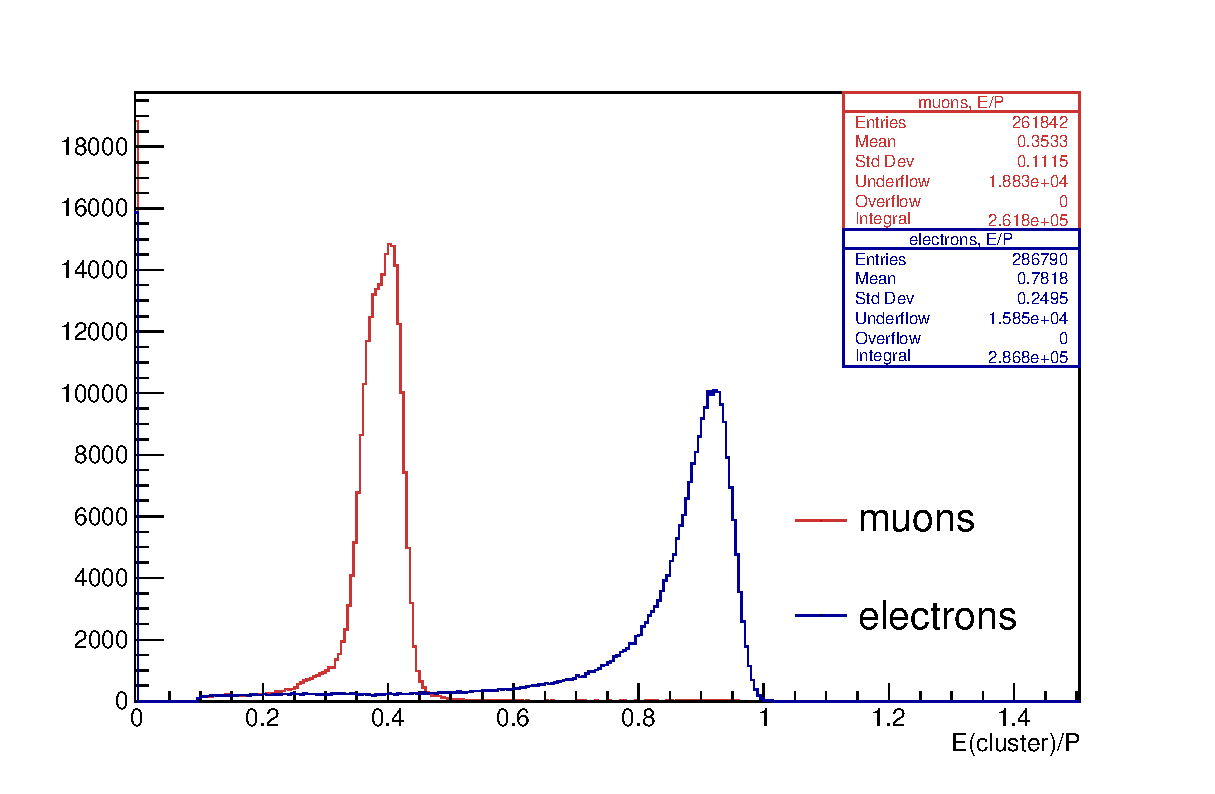
\includegraphics[width=0.50\textwidth]{figures/pdf/figure_00300_pid_emuana_1070_trk_101_ep}
    % }
    };
    \node[anchor=south west,inner sep=0] at (9.5,0.) {
      % \node[shift={(0 cm,0.cm)},inner sep=0,rotate={90}] at (0,0) {}
      % \makebox[\textwidth][c] {
      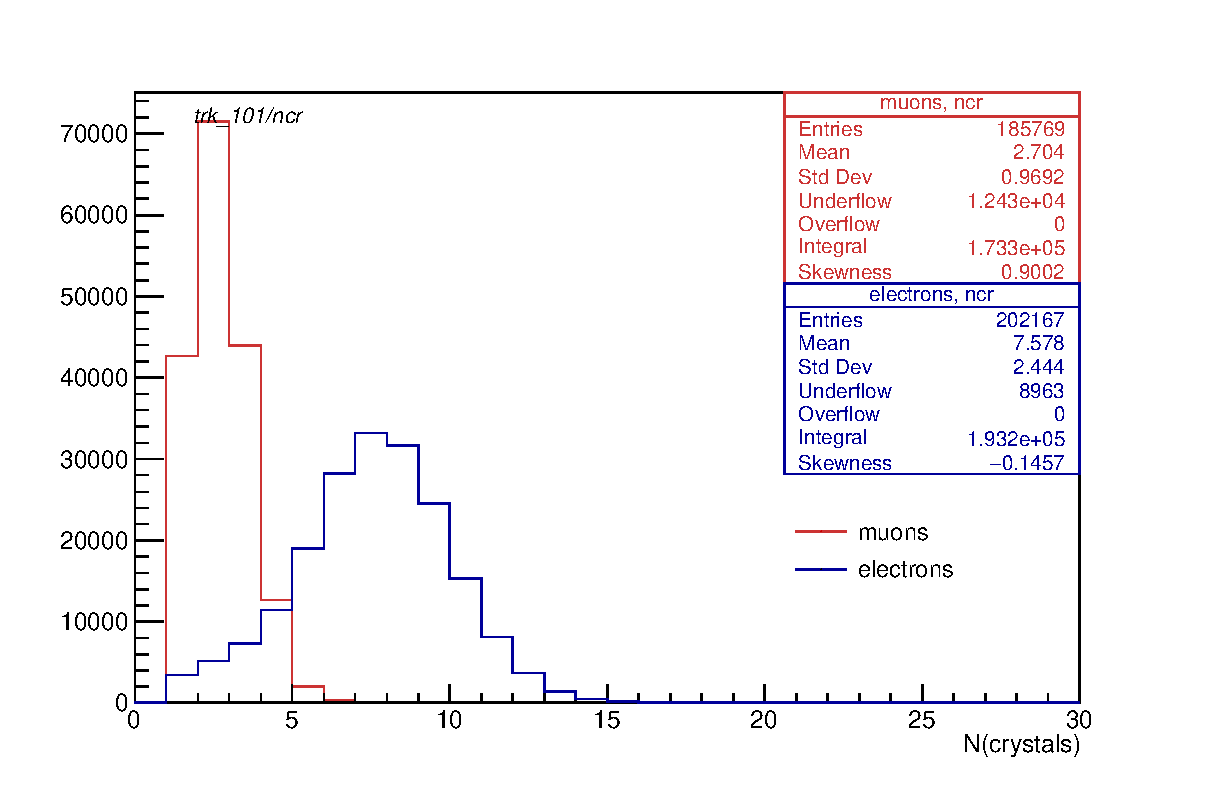
\includegraphics[width=0.50\textwidth]{figures/pdf/figure_00301_pid_emuana_1070_trk_101_ncr}
      % }
    };
    \node[anchor=south west,inner sep=0] at (-1,-6.) {
      % \node[shift={(0 cm,0.cm)},inner sep=0,rotate={90}] at (0,0) {}
      % \makebox[\textwidth][c] {
      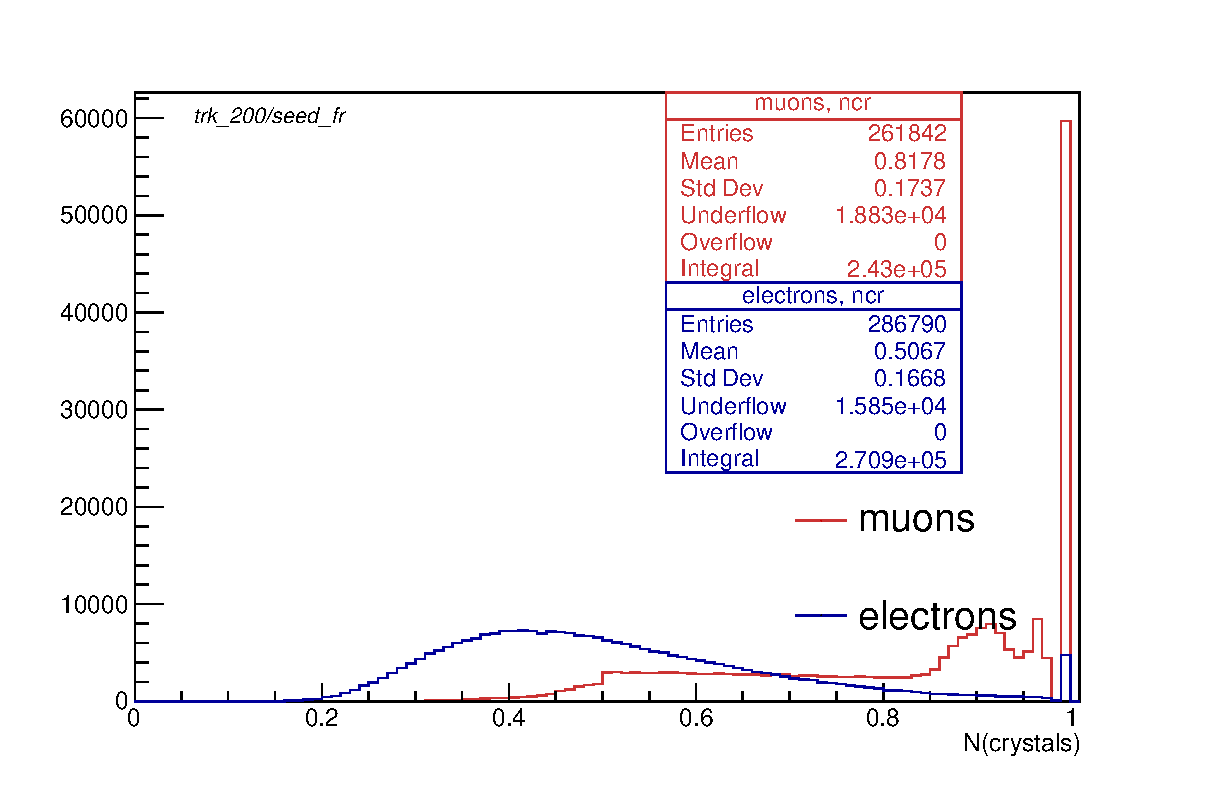
\includegraphics[width=0.50\textwidth]{figures/pdf/figure_00302_pid_emuana_1070_trk_101_seed_fr}
      % }
    };
    \node[anchor=south west,inner sep=0] at (9.5,-6.) {
      % \node[shift={(0 cm,0.cm)},inner sep=0,rotate={90}] at (0,0) {}
      % \makebox[\textwidth][c] {
      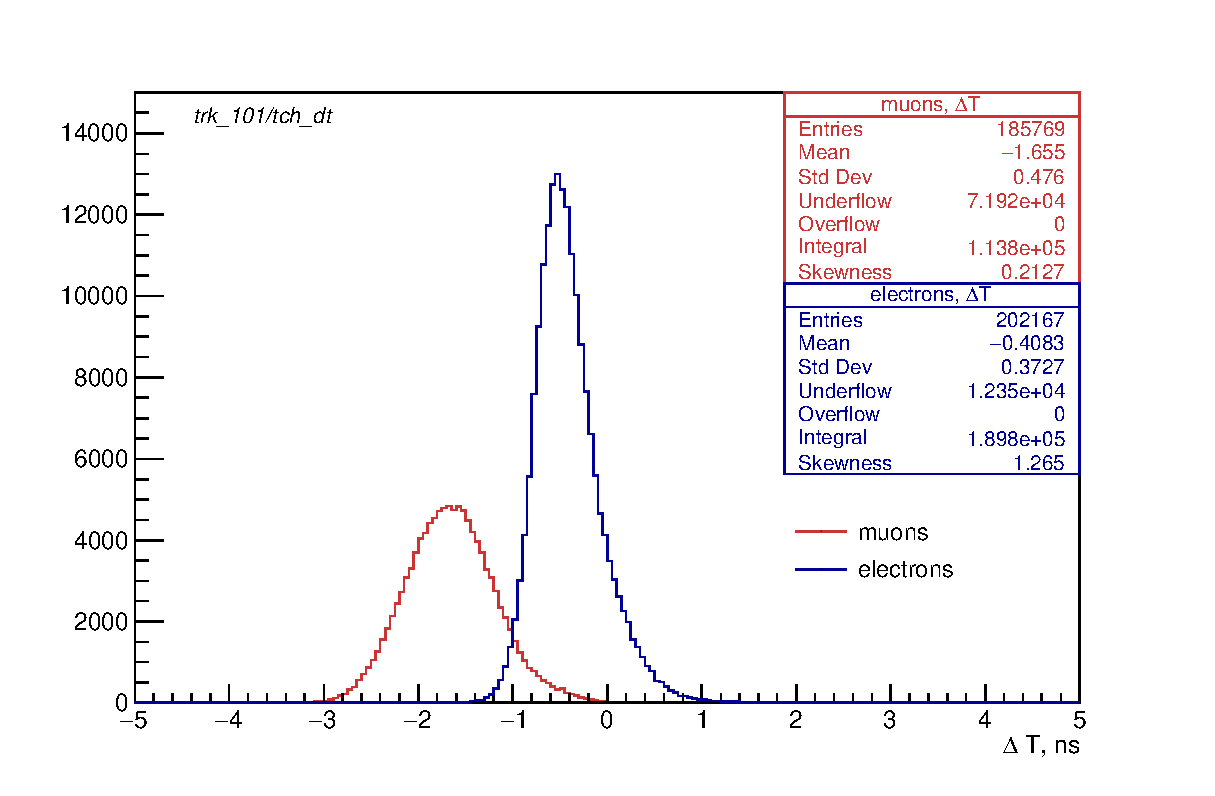
\includegraphics[width=0.50\textwidth]{figures/pdf/figure_00303_pid_emuana_1070_trk_101_tch_dt}
      % }
    };
    % \node [text width=6cm, scale=0.8] at (4.5,6.4) {mu2e-18894 by Kevin Lynch and Jim Popp};
  \end{tikzpicture}
  % \captionof{figure} {
  \caption{
    \label{fig:pid_training_1}
    The variables used in the PID ANN training: E/P, N(crystals), E(seed)/E, $\Delta T$
  }
\end{figure}

%%%%%%%%%% another figure
\begin{figure}[H]
  \hspace{-0.6in}
  \begin{tikzpicture}
    \node[anchor=south west,inner sep=0] at (0,0.) {
      % \node[shift={(0 cm,0.cm)},inner sep=0,rotate={90}] at (0,0) {}
      % \makebox[\textwidth][c] {
      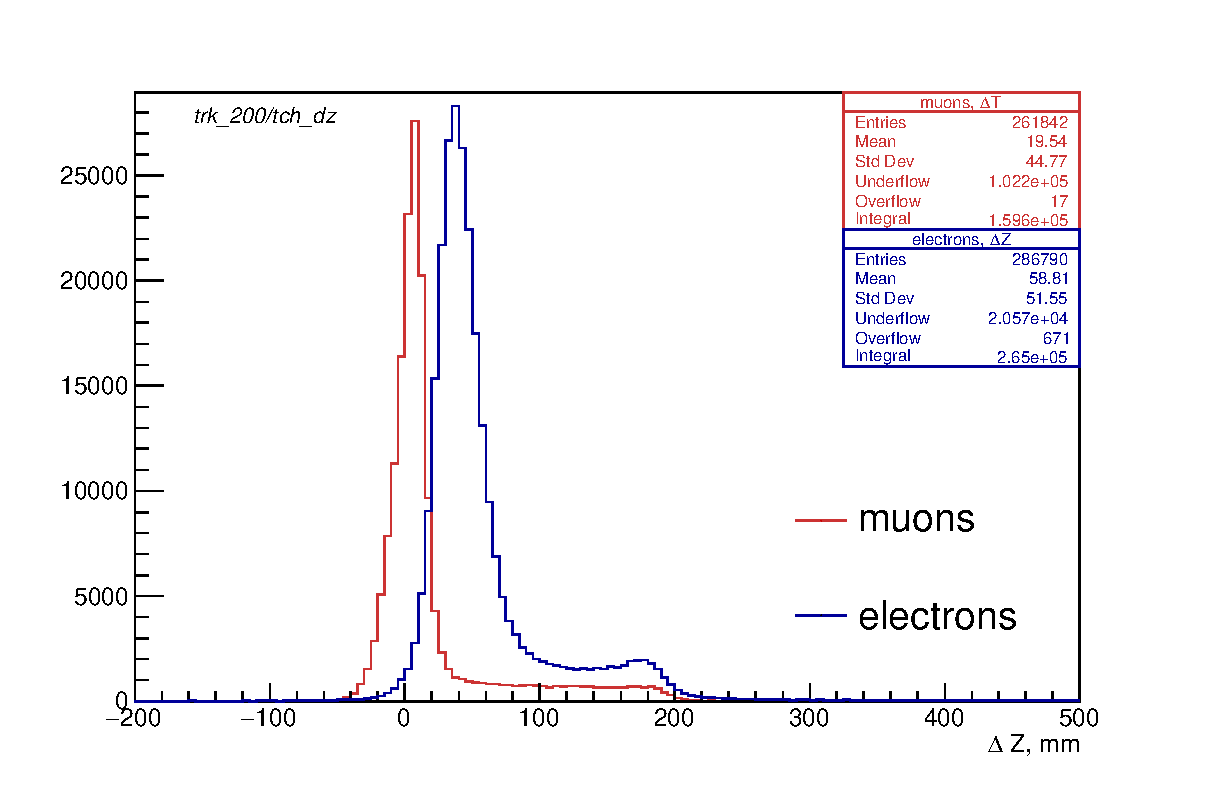
\includegraphics[width=0.50\textwidth]{figures/pdf/figure_00304_pid_emuana_1070_trk_101_tch_dz}
      % }
    };
    \node[anchor=south west,inner sep=0] at (10.5,0) {
      % \node[shift={(0 cm,0.cm)},inner sep=0,rotate={90}] at (0,0) {}
      % \makebox[\textwidth][c] {
      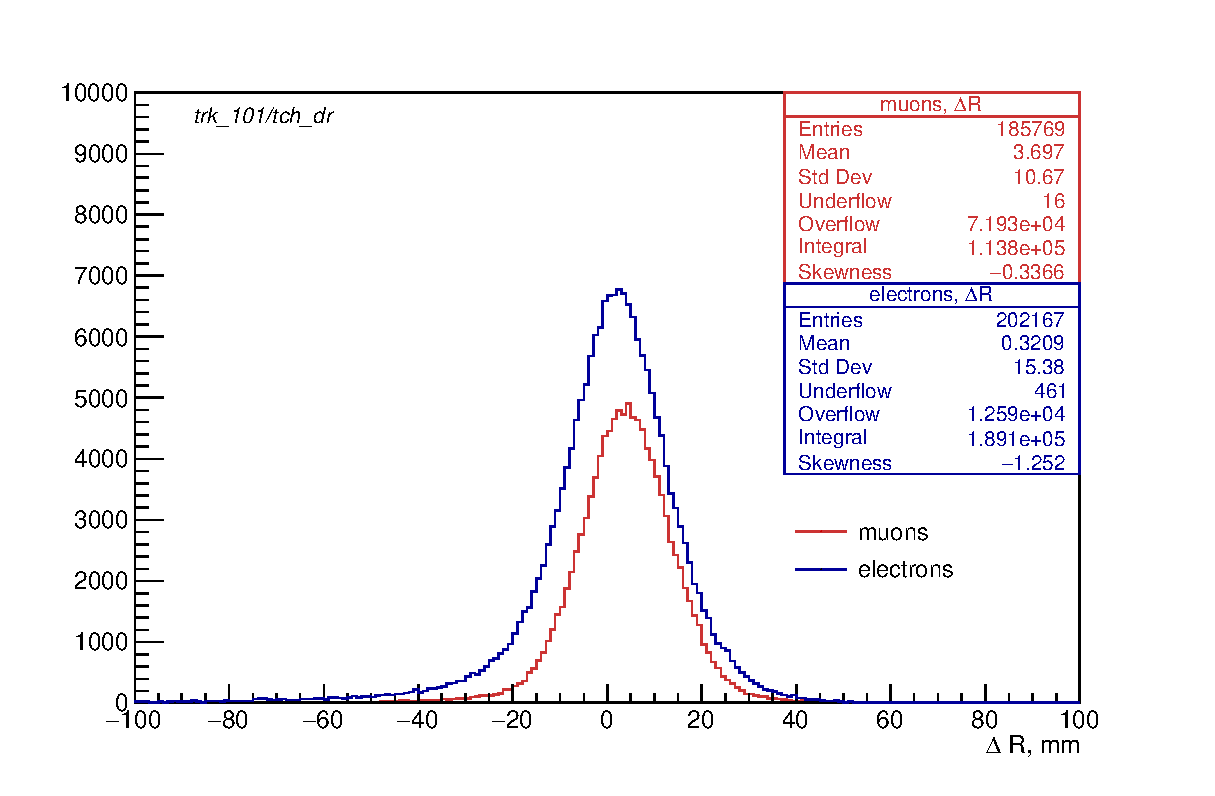
\includegraphics[width=0.50\textwidth]{figures/pdf/figure_00305_pid_emuana_1070_trk_101_tch_dr}
      % }
    };
    \node[anchor=south west,inner sep=0] at (0.,-6) {
      % \node[shift={(0 cm,0.cm)},inner sep=0,rotate={90}] at (0,0) {}
      % \makebox[\textwidth][c] {
      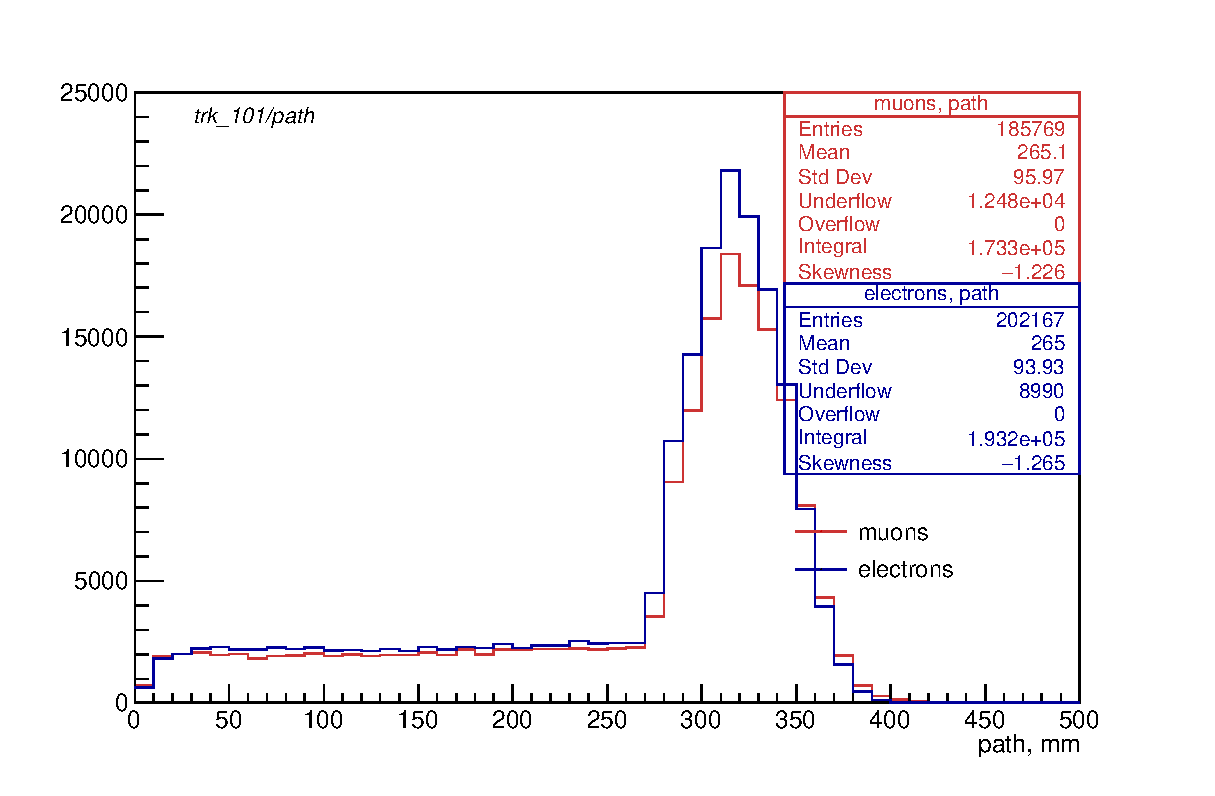
\includegraphics[width=0.50\textwidth]{figures/pdf/figure_00306_pid_emuana_1070_trk_101_path}
      % }
    };
    % \node [text width=6cm, scale=0.8] at (4.5,6.4) {mu2e-18894 by Kevin Lynch and Jim Popp};
  \end{tikzpicture}
  %% \captionof{figure} {
    \caption{
    \label{fig:pid_training_2}
    The variables used in the PID ANN training: $\Delta Z$, $\Delta R$, path
  }
\end{figure}


Results of the PID ANN training are shown in Figure \ref{fig:pid_training_3}. 
From the training plots, one might conclude that the separation between the
electrons and muons provided by the ANN is close to perfect. 
To identify 105 MeV electrons, we require the PID ANN score $S_{PID} > 0.5$.
The PID ANN training is validated by running the PID algorithm on the full ele00s61b0 and mumi0s51b0 datasets.
The datasets have about 200K events each, including events used for training.
The results presented in Figure \ref{fig:pid_training_4} show that the efficiency of a $S_{PID} > 0.5$ cut 
for electrons is about 99.2\%, and about 0.8\% of muons are mis-identified as electrons.
The spike at 1 in the ANN score distribution for muons corresponds to muon decays in flight,
where the particle reconstructed in the event is an electron.
Remaining sources of muon mis-identification will be studied in detail later.
To identify 105 MeV electrons for SU2020 analyses, we require a PID ANN score of $S_{PID} > 0.5$.


\begin{figure}[H]
\hspace{-0.6in}
  \begin{tikzpicture}
    \node[anchor=south west,inner sep=0] at (0,0.) {
      % \node[shift={(0 cm,0.cm)},inner sep=0,rotate={90}] at (0,0) {}
      % \makebox[\textwidth][c] {
      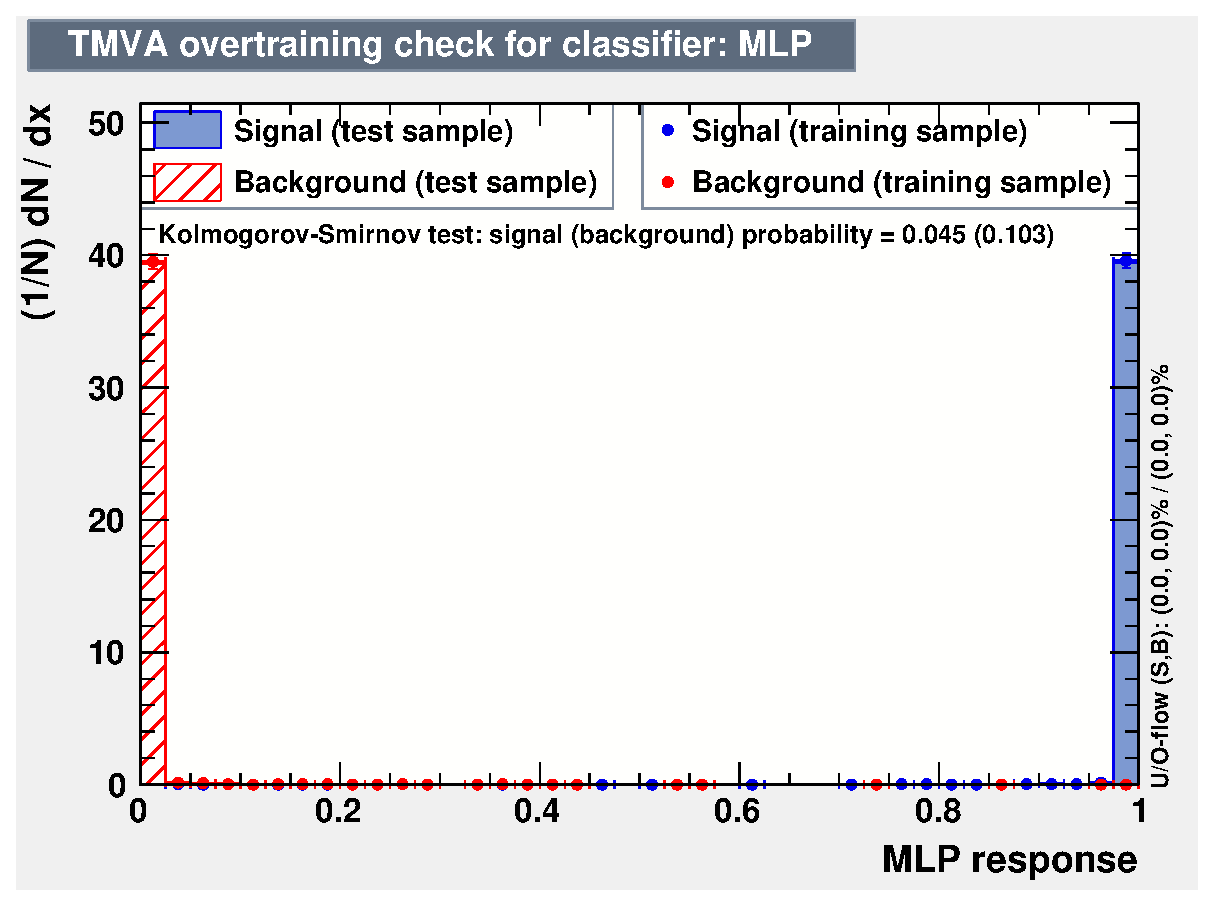
\includegraphics[width=0.55\textwidth]{figures/pdf/pid_mva_overtrain_mlp}
      % }
    };
    \node[anchor=south west,inner sep=0] at (10.5,0.5) {
      % \node[shift={(0 cm,0.cm)},inner sep=0,rotate={90}] at (0,0) {}
      % \makebox[\textwidth][c] {
      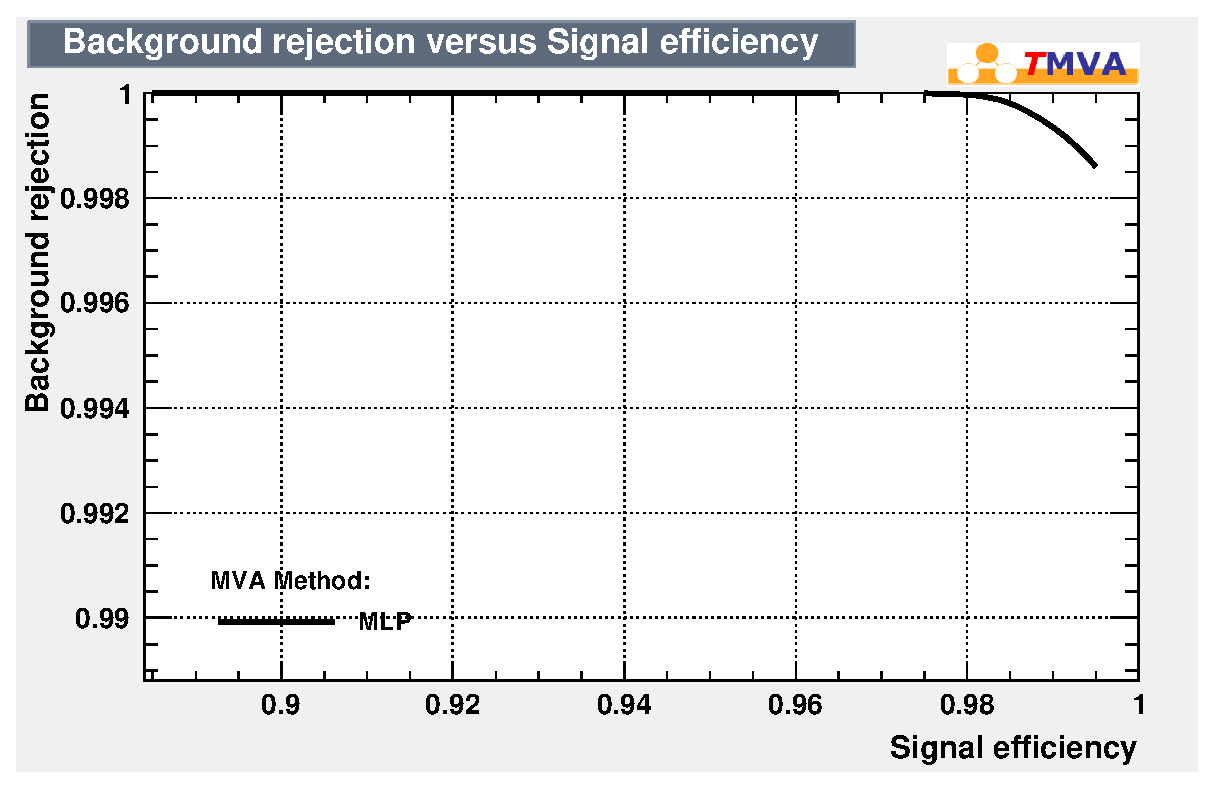
\includegraphics[width=0.55\textwidth]{figures/pdf/pid_mva_rejection_mlp}
      % }
    };
    % \node [text width=6cm, scale=0.8] at (4.5,6.4) {mu2e-18894 by Kevin Lynch and Jim Popp};
  \end{tikzpicture}
  % \captionof{figure} {
  \caption{
    \label{fig:pid_training_3}
    The output of the PID ANN training: overtraining check on the left and efficiency vs rejection 
    on the right
  }
\end{figure}

\begin{figure}[H]
  \begin{tikzpicture}
    \node[anchor=south west,inner sep=0] at (0,0.) {
      % \node[shift={(0 cm,0.cm)},inner sep=0,rotate={90}] at (0,0) {}
      \makebox[\textwidth][c] {
        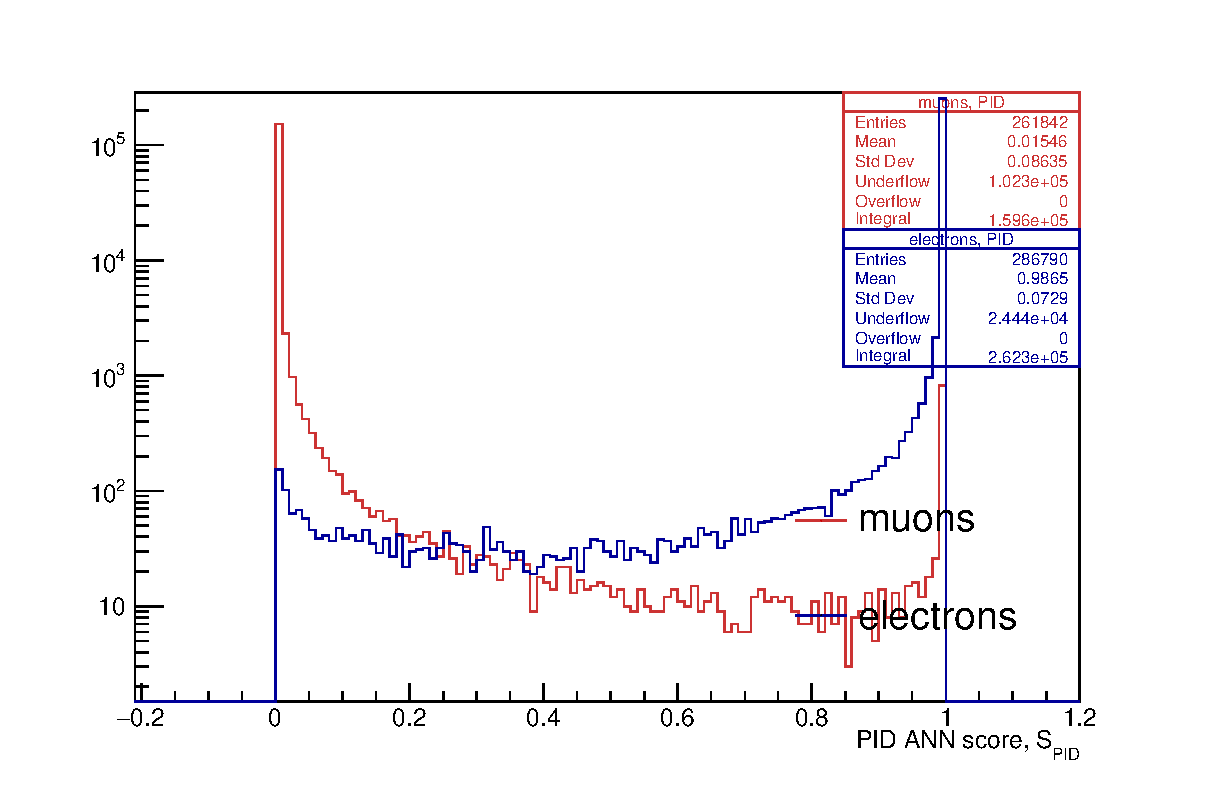
\includegraphics[width=1.0\textwidth]{figures/pdf/figure_00307_pid_emuana_1070_trk_101_pidmvaout}
      }
    };
    % \node [text width=6cm, scale=0.8] at (4.5,6.4) {mu2e-18894 by Kevin Lynch and Jim Popp};
  \end{tikzpicture}
  % \captionof{figure} {
  \caption{
    \label{fig:pid_training_4}
    Distribution in the PID ANN score for electron and muon samples, samples include events used for training,
    10000 events each. A spike in muon PID at 1  - muon decays in flight. \\ 
    % {\color{red} \bf check that underflows are events without clusters}
  }
\end{figure}

The efficiencies of the PID preselection cuts for the {\bf cele0s61b1} dataset are listed
in Table \ref{tab:pid_preselection_cuts}. The total preselection efficiency is about 93\%.
%
Out of that, approximately, 96\% comes from the requirement on the calorimeter cluster that E > 10 MeV
to be reconstructed in an event. Therefore, for events with the reconstructed track with $P > 100$ MeV/c 
and a reconstructed cluster, efficiency of the PID preselection is 96.7 \%

% Q: how does 96\% of the inefficiency come from the cluster requirement, but after this efficiency is still 96.7\%?.
% A: 0.96*0.967 = 0.93

For single track 105 MeV/c electron events passing the PID preselection, the efficiency
of the $S_{PID} > 0.5$ cut is 99.3\% .
\begin{table}[H]
  \begin{center}
    \begin{tabular}{l|c|c} % <-- Changed to S here.
      \textbf{Cut}                    & \textbf{N events after } & \textbf{Efficiency }\\
      \hline
      Number generated events         & 1000000                  &            \\
      total number of tracks          &  329715                  &   0.330    \\
      \hline                                                     
      track passes TID cuts           &  193252                  &   0.586    \\
      $P > 100$ MeV/c                 &  178078                  &   0.921    \\
      $|\Delta{T}| < 10$ ns           &  167028                  &   0.937     \\
      $-50 < dz < 250$                &  164951                  &   0.988    \\
      $ E/P < 1.2$                    &  164884                  &   1.000    \\
      \hline                                                     
      $S_{PID} >0.5$                   &  163543                  &   0.992    \\
   \end{tabular}
  \end{center}
  \caption{
    \label{tab:pid_preselection_cuts}
    The PID preselection cuts (defined using {\bf ele00s61b0} ) and the efficiency for {\bf cele0s51b1} electrons.
    TID cuts refers to the track ID cuts for the $\MuToEm$ channel.
    \\
    % {\red check which dataset the efficiencies are given for} 
  }
\end{table}

Out of 109004 muons with $P > 100$ MeV/c and passing the preselection cuts, 776 have a PID ANN score $S_{PID} > 0.5$,
which corresponds to a fake rate of about 0.7\%. Leading contributions to that rate come from muon decays in flight 
and decays of stopped muons in the calorimeter.

%%%%%%%%%%%%%%%%%%%%%%%%%%%%%%%%%%%%%%%%%%%%%%%%%%%%%%%%%%%%%%%%%%%%%%%%%%%%%%
\subsection { Electrons failing the PID selection}
\label{sec:electrons_failing_pid}

Figure \ref{fig:electrons_failing_pid} compares distributions of some ID variables for electrons 
passing and failing the PID cuts.
%
Although only 0.8\%  of events are in question, understanding of the ANN failures could help finding 
reconstruction problems.
\begin{itemize}
\item 
  {\red Of special interest seems to be the spike in the distribution in $R_{max}$ - to be investigated}
\item
  {\red also electrons with $\Delta{T} < -1.5$ ns - to be investigated}
\end{itemize}

\begin{figure}[H]
\hspace{-0.6in}
  \begin{tikzpicture}
    \node[anchor=south west,inner sep=0] at (0,0.) {
      % \node[shift={(0 cm,0.cm)},inner sep=0,rotate={90}] at (0,0) {}
      % \makebox[\textwidth][c] {
      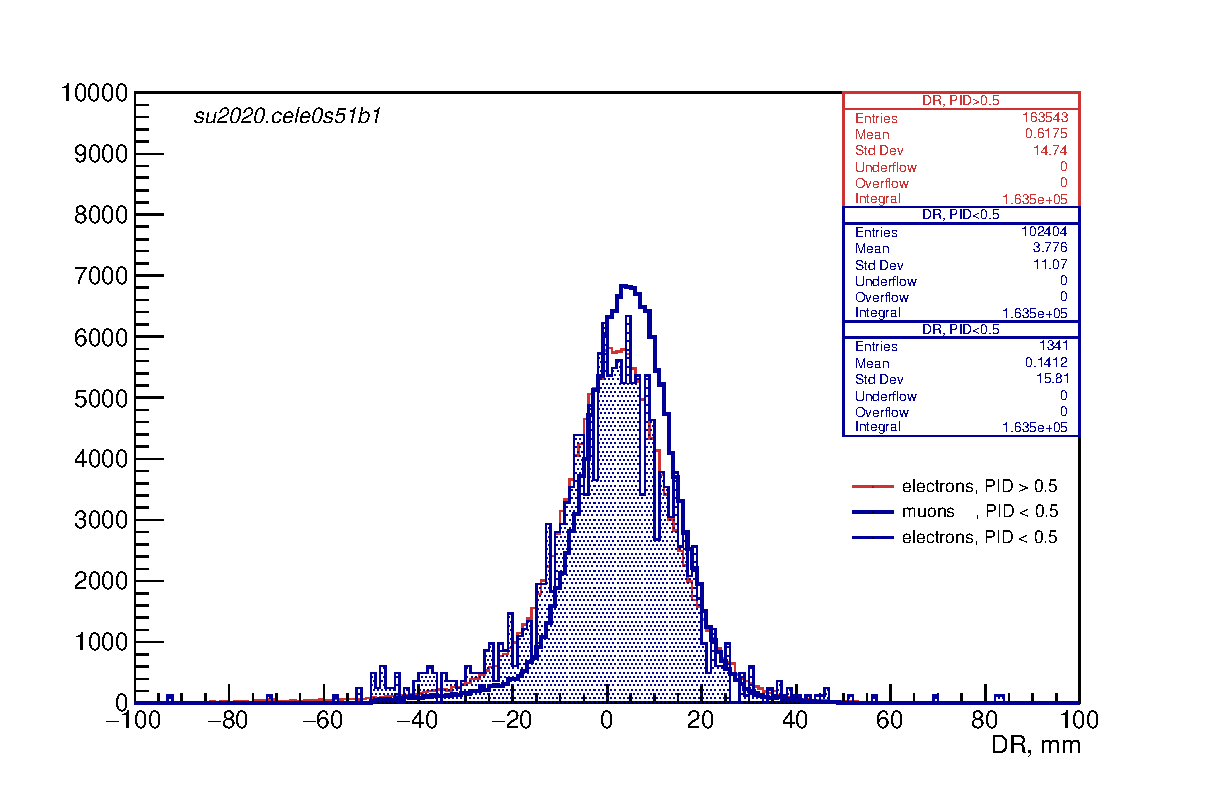
\includegraphics[width=0.60\textwidth]{figures/pdf/figure_00310_pid_emuana_trk_110_vs_111_tch_dr}
      % }
    };
    \node[anchor=south west,inner sep=0] at (10.3,0.) {
      % \node[shift={(0 cm,0.cm)},inner sep=0,rotate={90}] at (0,0) {}
      % \makebox[\textwidth][c] {
      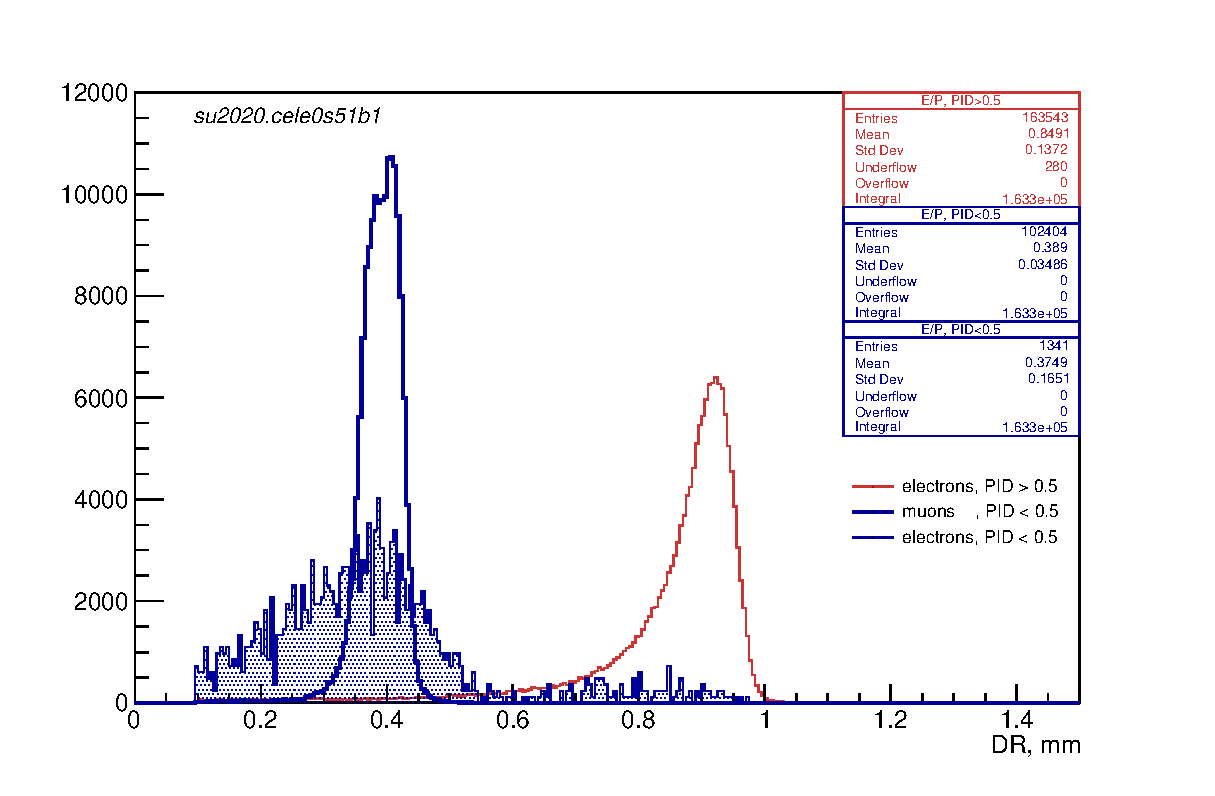
\includegraphics[width=0.60\textwidth]{figures/pdf/figure_00311_pid_emuana_trk_110_vs_111_ep}
      % }
    };
    \node[anchor=south west,inner sep=0] at (0,-7.0) {
      % \node[shift={(0 cm,0.cm)},inner sep=0,rotate={90}] at (0,0) {}
      % \makebox[\textwidth][c] {
      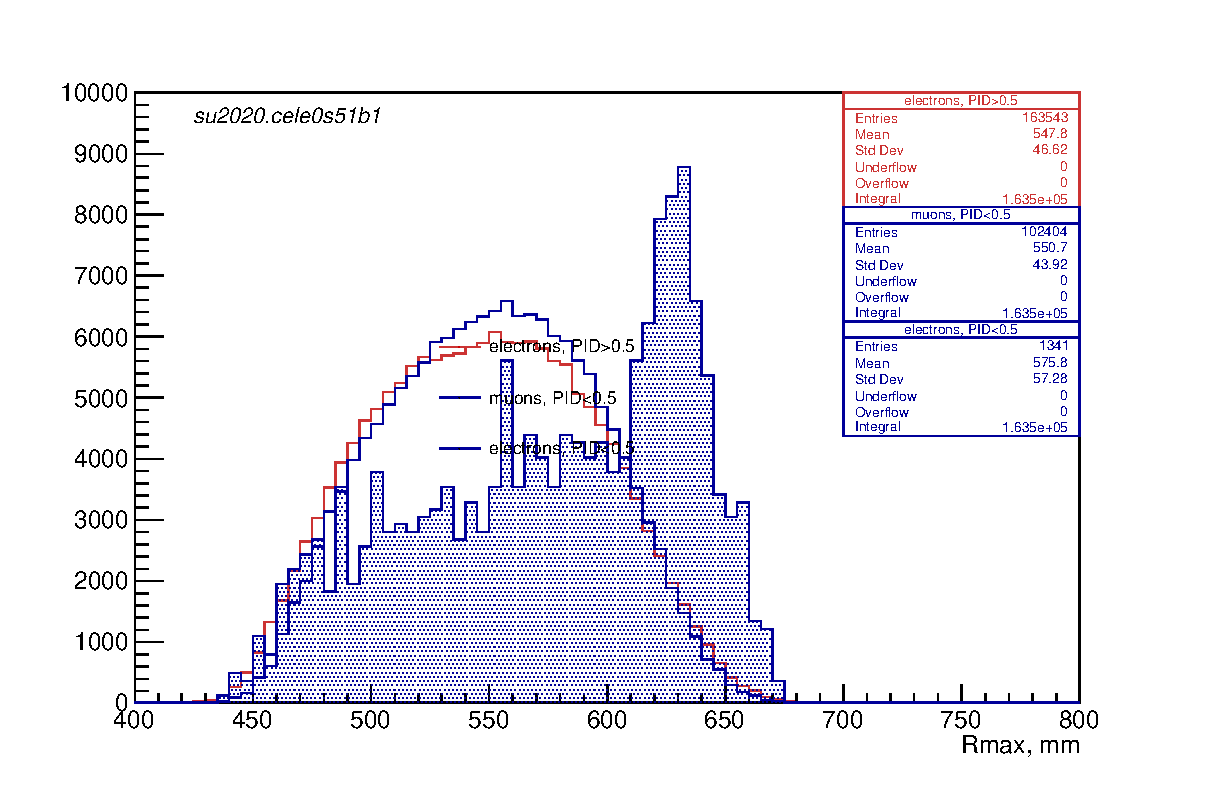
\includegraphics[width=0.60\textwidth]{figures/pdf/figure_00312_pid_emuana_trk_110_vs_111_rmax}
      % }
    };
    \node[anchor=south west,inner sep=0] at (10.3,-7.0) {
      % \node[shift={(0 cm,0.cm)},inner sep=0,rotate={90}] at (0,0) {}
      % \makebox[\textwidth][c] {
      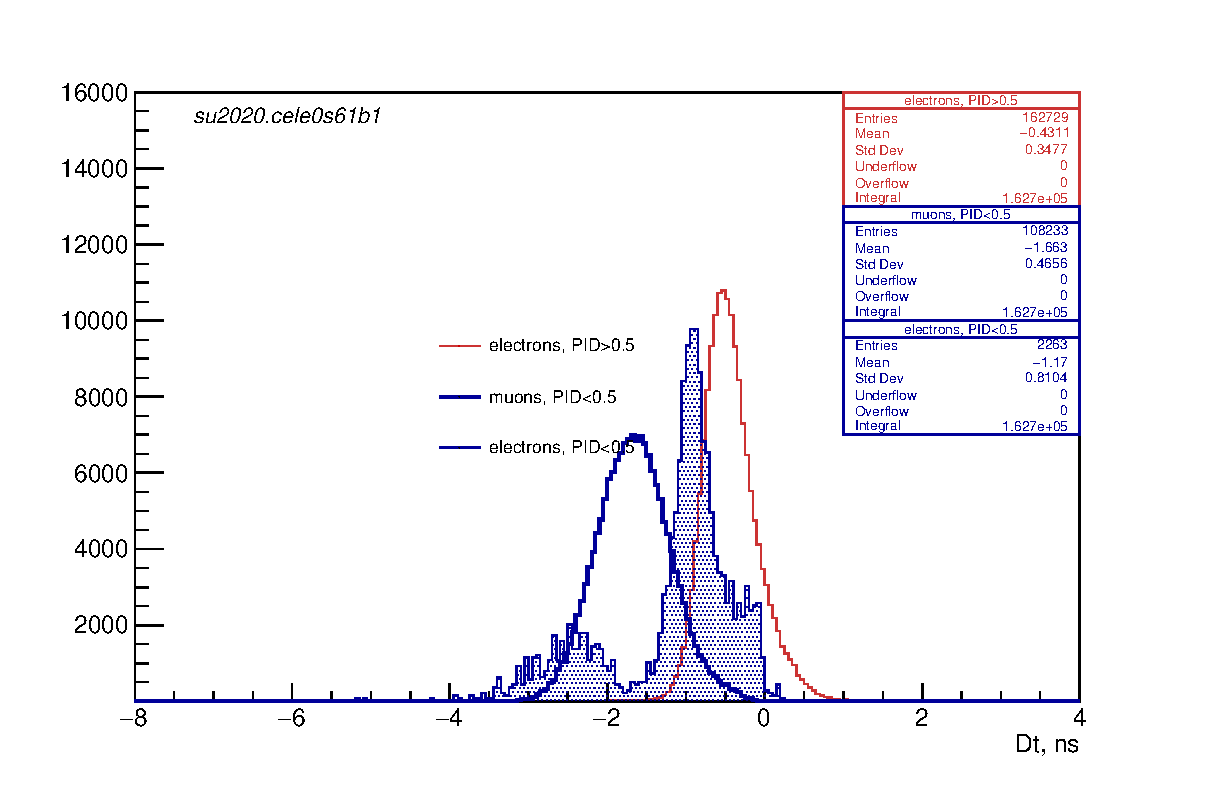
\includegraphics[width=0.60\textwidth]{figures/pdf/figure_00313_pid_emuana_trk_110_vs_111_tch_dt}
      % }
    };
    % \node [text width=6cm, scale=0.8] at (4.5,6.4) {mu2e-18894 by Kevin Lynch and Jim Popp};
  \end{tikzpicture}
  \captionof{figure} {
    \label{fig:electrons_failing_pid}
    % \caption{
    Distributions of the PID variables for electrons passing the PID, muons failing the PID, and electrons failing the PID.
    The PID selection used is $S_{PID} > 0.5$, where $S_{PID}$ is the value of the PID ANN score variable
  }
\end{figure}


%%%%%%%%%%%%%%%%%%%%%%%%%%%%%%%%%%%%%%%%%%%%%%%%%%%%%%%%%%%%%%%%%%%%%%%%%%%%%%
\newpage
\subsection{\MuToEp\ channel}
\label{sec:mumep_channel_pid}
% {\blue lowercase title words after first word}

The PID in \MuToEp\ channel uses a similar ANN trained  using  92 MeV/c positrons and 
positive muons from {\bf pos01s51b0} and {\bf mupl1s51b0} datasets respectively. 
The training procedure is the same as described in Section \ref{sec:mumem_pid_ann_training}.
% 
Figure \ref{fig:pid_score_mumep} shows distributions of the PID ANN score, $S_{PID}$,
for 92 MeV/c positrons and positive muons. About 1.2\% of all muon events have $S_{PID} > 0.5$,
more than 50\% of those events are positrons produced in muon decays in flight.

Plotting the data in log scale - see Figure \ref{fig:pid_score_mumep}(b) - reveals a spike around 0.25,
present in both positron and muon distributions.

% {\red Although the relative contribution of the spike is small, its origin needs to be investigated.}

\begin{figure}[H]
\hspace{-0.6in}
  \begin{tikzpicture}
    \node[anchor=south west,inner sep=0] at (0,0.) {
      % \node[shift={(0 cm,0.cm)},inner sep=0,rotate={90}] at (0,0) {}
      % \makebox[\textwidth][c] {
      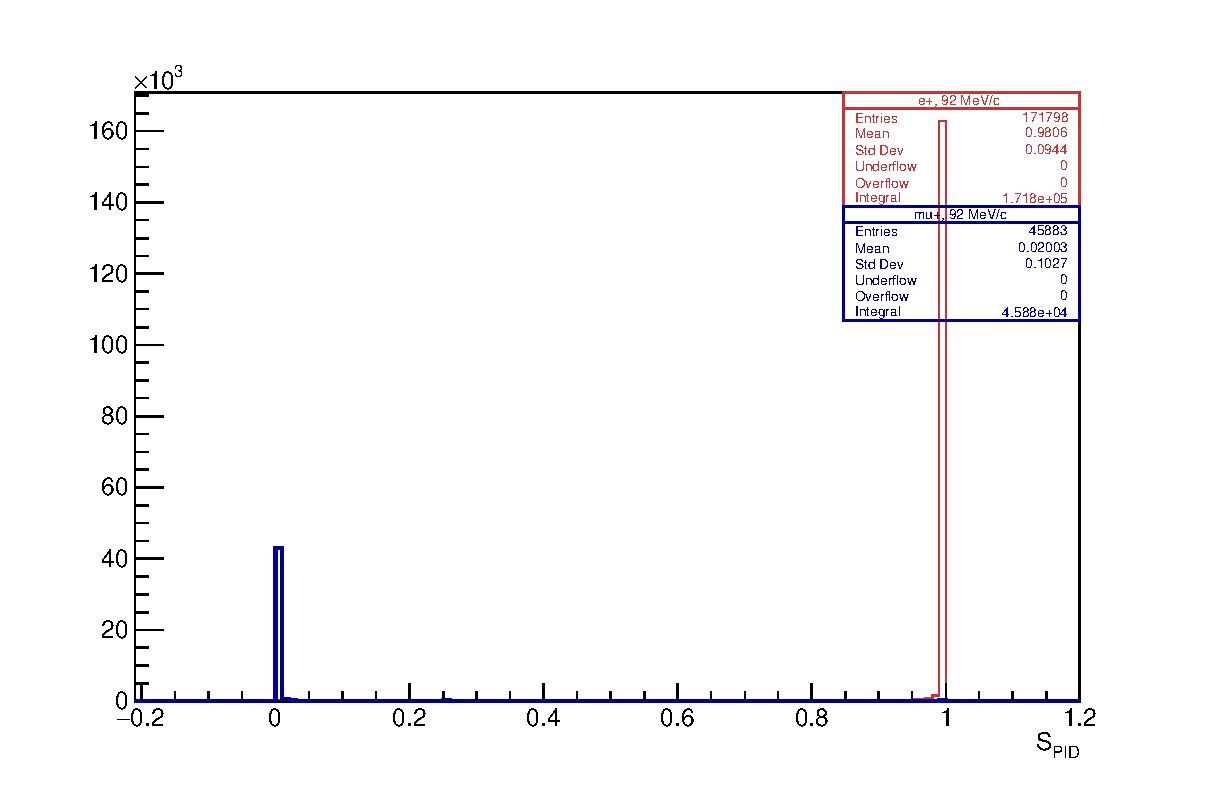
\includegraphics[width=0.60\textwidth]{figures/pdf/figure_00331_su2020_track_ana_1110_trk_219_pidmvaout}
      % }
    };
    \node [text width=1cm, scale=1.0] at (3.,4.5) {(a)};
    \node[anchor=south west,inner sep=0] at (10.5,0.) {
      % \node[shift={(0 cm,0.cm)},inner sep=0,rotate={90}] at (0,0) {}
      % \makebox[\textwidth][c] {
      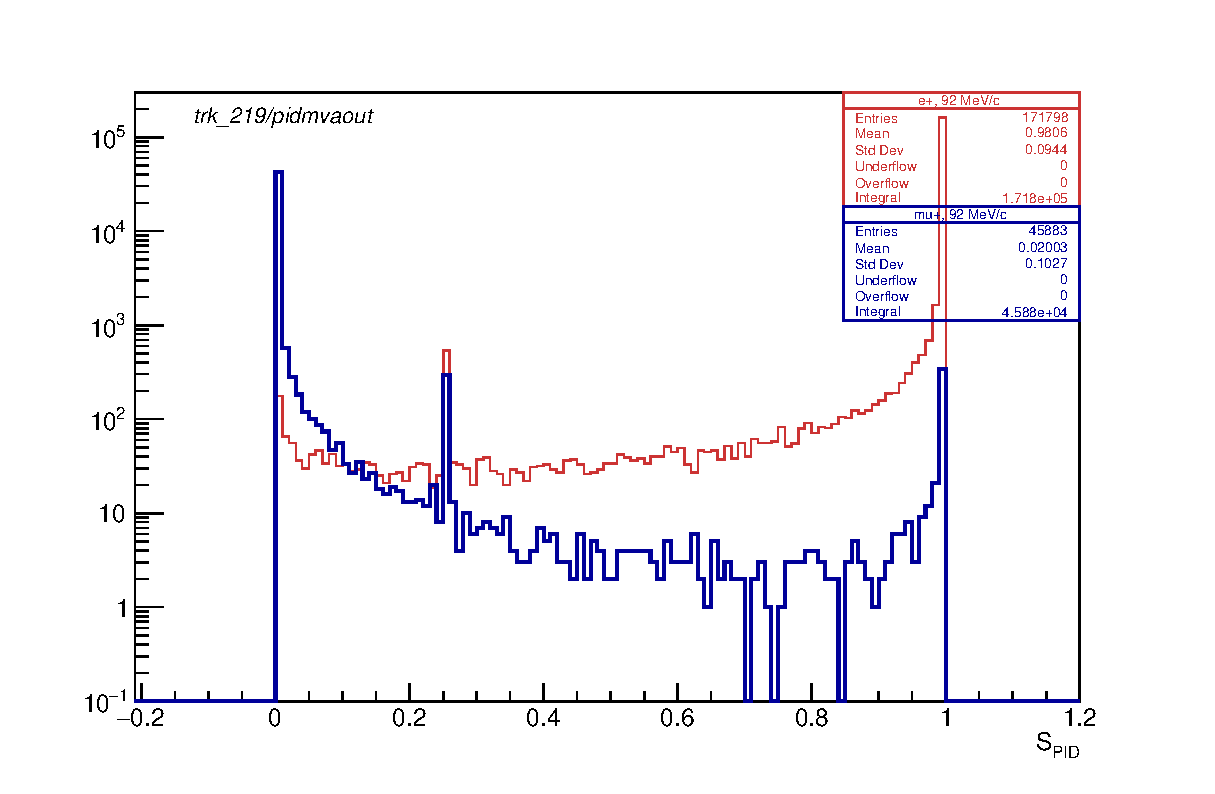
\includegraphics[width=0.60\textwidth]{figures/pdf/figure_00332_su2020_track_ana_1110_trk_219_pidmvaout_log}
      % }
    };
    \node [text width=1cm, scale=1.0] at (13.5,4.5) {(b)};
  \end{tikzpicture}
  \captionof{figure} {
    \label{fig:pid_score_mumep}
    The results of the PID ANN training for the \MuToEp\ channel: the distribution of the PID ANN score, $S_{PID}$,
    for single 92.3 MeV/c positrons and positive muons; (a): linear scale; (b): log scale. \\
    {\red Nature of the spike around 0.25 needs to be investigated.}
  }
\end{figure}
